\begin{figure}
\centering
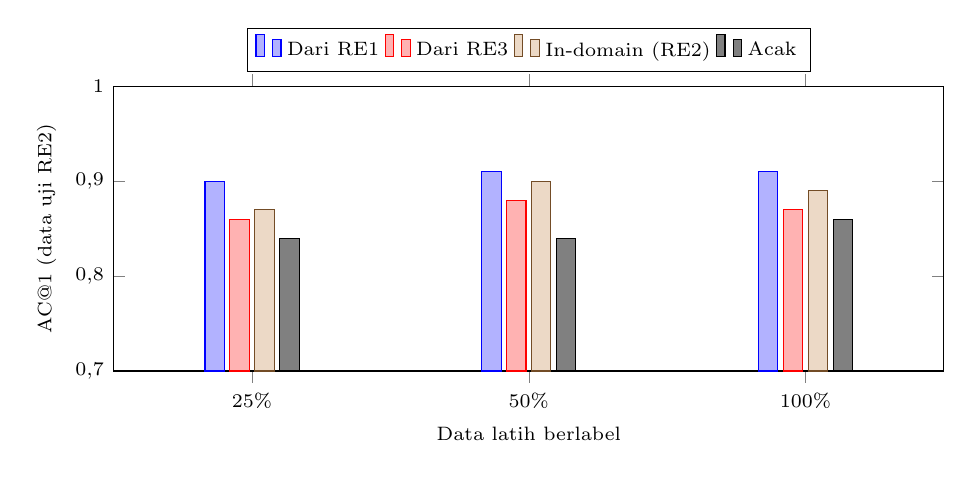
\begin{tikzpicture}
\begin{axis}[
  ybar, bar width=7pt, width=\textwidth, height=5.2cm,
  ymin=0.7, ymax=1.0, ylabel={AC@1 (data uji RE2)},
  yticklabel style={/pgf/number format/.cd, fixed, precision=1, use comma},
  scaled y ticks=false,
  symbolic x coords={p25,p50,p100}, xtick=data,
  xticklabels={25\%,50\%,100\%},
  xlabel={Data latih berlabel},
  legend style={at={(0.5,1.05)},anchor=south,legend columns=-1,font=\scriptsize},
  tick label style={font=\scriptsize}, label style={font=\scriptsize},
  enlarge x limits=0.25]
\addplot coordinates {(p25,0.90) (p50,0.91) (p100,0.91)};
\addplot coordinates {(p25,0.86) (p50,0.88) (p100,0.87)};
\addplot coordinates {(p25,0.87) (p50,0.90) (p100,0.89)};
\addplot coordinates {(p25,0.84) (p50,0.84) (p100,0.86)};
\legend{Dari RE1, Dari RE3, In-domain (RE2), Acak}
\end{axis}
\end{tikzpicture}
\caption{EX-2, TS2Vec, FineLast: AC@1 pada RE2 menurut fraksi data latih berlabel (nilai dari slide proyek, rata-rata 3 seed). Heuristik memperoleh 0,80 pada RE2; sumbu-y dimulai dari 0,7. Seri TimeMAE dan RUN-encoder akan ditambahkan ketika eksperimennya tersedia.}\label{fig:ex2}
\end{figure}
